%%% Presentaciones para Lenguajes de programacion y sus paradigmas 

\documentclass[xcolor=dvipsnames,table,handout]{beamer}
%\documentclass[xcolor=dvipsnames,table]{beamer}

\newcommand{\espc}{\vspace{0.3cm}}

\usepackage[utf8]{inputenc}
\usepackage[spanish]{babel}
\usepackage{hyperref}
\usepackage{lmodern}
\usepackage[T1]{fontenc}

%%%% paquetes matematicas
\usepackage{amssymb,amsmath,amscd}
\usepackage{extarrows}
\usepackage{stmaryrd}
\usepackage{mathabx}
\usepackage{mathrsfs}
% \usepackage{mathabx}
\usepackage{amsthm}

%%%%%
\usepackage{hyperref}
\usepackage{graphicx}
\usepackage{multicol}
\usepackage{pifont}
\usepackage{xcolor}
\usepackage{etex}
\usepackage{tikz}
\usepackage{array}
%\usepackage{pgfplots}

%%%% cosmetics
% D.Remy package for pretty display of rules
\usepackage{mathpartir}

% para insertar codigo con formato particular 
\usepackage{listing} 

% comillas 
\usepackage[autostyle=true,spanish=mexican]{csquotes}

% codigo 
\usepackage{verbatim}
\usepackage{alltt}

% footnotes
\usepackage[bottom]{footmisc}
\usepackage{setspace}

\usepackage{wrapfig}
\usepackage{caption}


\hfuzz=5.002pt %parameter to allow hbox overfulled by length before error!

% Options for presentation
% ------------------------
% \definecolor{mycolor}{RGB}{255,192,3}
\definecolor{mycolor}{RGB}{17,132,221}
\mode<presentation>
{
% \usetheme[secheader]{Boadilla}
% \usecolortheme{orchid}
\useoutertheme{infolines}
\useinnertheme{rectangles}
\setbeamertemplate{itemize items}[square]
\setbeamertemplate{enumerate items}[square]
\setbeamersize{text margin left=6mm, text margin right=6mm}

\setbeamercolor{alerted text}{fg=red,bg=red!70!white}
\setbeamercolor{background canvas}{bg=white}
\setbeamercolor{frametitle}{bg=mycolor,fg=white}
\setbeamercolor{normal text}{bg=white,fg=black}
\setbeamercolor{structure}{bg=black,fg=mycolor}
\setbeamercolor{title}{bg=mycolor,fg=white}
\setbeamercolor{subtitle}{bg=mycolor,fg=white}
\setbeamercolor{titlelike}{bg=white,fg=mycolor}

\setbeamercovered{invisible}

\setbeamercolor*{palette primary}{fg=mycolor,bg=white}
\setbeamercolor*{palette secondary}{bg=white,fg=white}
\setbeamercolor*{palette tertiary}{fg=mycolor,bg=white}
\setbeamercolor*{palette quaternary}{fg=white,bg=white}

\setbeamercolor{separation line}{bg=mycolor,fg=mycolor}
\setbeamercolor{fine separation line}{bg=white,fg=red}
\setbeamercolor{author in head/foot}{bg=mycolor!30!white,fg=mycolor!80!black}
\setbeamercolor{title in head/foot}{bg=mycolor!30!white,fg=mycolor!80!black}
\setbeamercolor{date in head/foot}{bg=mycolor!30!white,fg=mycolor!80!black}
\setbeamercolor{institute in head/foot}{bg=mycolor!30!white,fg=mycolor!80!black}
\setbeamercolor{section in head/foot}{bg=mycolor!60!white, fg=Red}
\setbeamercolor{subsection in head/foot}
{bg=mycolor!50!white,fg=mycolor!50!white}


\setbeamertemplate{headline}
{
  \leavevmode%
  \hbox{%
  \begin{beamercolorbox}[wd=.5\paperwidth,ht=2.65ex,dp=1.5ex,center]{section in 
head/foot}%
    \usebeamerfont{section in head/foot}\insertsectionhead\hspace*{2ex}
  \end{beamercolorbox}%
  \begin{beamercolorbox}[wd=.5\paperwidth,ht=2.65ex,dp=1.5ex,center]{subsection 
in head/foot}%
    \usebeamerfont{subsection in head/foot}\hspace*{2ex}\insertsubsectionhead
  \end{beamercolorbox}}%
  \vskip0pt%
}
% \beamerdefaultoverlayspecification{<+->}
\beamertemplatenavigationsymbolsempty
% \setbeamertemplate{footline}[frame number]
}

%%%% Macros para las notas de lenguajes de programacion


%%%% math

\newcommand{\vphi}{\varphi}
\newcommand{\vp}{\varphi}

% \newcommand{\dn}{\mathsf{DN}}
% \newcommand{\dnC}{\mathsf{DN_C}}
% \newcommand{\dnM}{\mathsf{DN_M}}
% \newcommand{\dnp}{\mathsf{DN_p}}
% \newcommand{\dnm}{\mathsf{DN_p^M}}
% \newcommand{\dnc}{\mathsf{DN_p^C}}

%\newcommand{\case}{\mathsf{case}}
%\renewcommand\labelitemi{$\circ$}

\newcommand{\imp}{\rightarrow}
\newcommand{\Imp}{\Rightarrow}
\renewcommand{\iff}{\leftrightarrow}
\newcommand{\Iff}{\Leftrightarrow}
\newcommand{\G}{\Gamma}
\newcommand{\D}{\Delta}


\newcommand{\De}{\mathcal{D}}
\newcommand{\F}{\mathcal{F}}
\newcommand{\Ge}{\mathcal{G}}
\newcommand{\Pe}{\mathcal{P}}
\newcommand{\I}{\mathcal{I}}
\newcommand{\C}{\mathcal{C}}
\newcommand{\K}{\mathcal{K}}
\renewcommand{\L}{\mathcal{L}}
\newcommand{\M}{\mathcal{M}}
\newcommand{\Nc}{\mathcal{N}}
%\newcommand{\E}{\mathcal{E}}
%\newcommand{\R}{\mathcal{R}}
%\newcommand{\Q}{\mathcal{Q}}
\newcommand{\Sc}{\mathcal{S}}
\newcommand{\Te}{\mathcal{T}}
\newcommand{\W}{\mathcal{W}}

\newcommand{\Db}{\mathbb{D}}
\newcommand{\Fb}{\mathbb{F}}
\newcommand{\Kb}{\mathbb{K}}
\newcommand{\Eb}{\mathbb{E}}
\newcommand{\Ebs}{\mathbb{E}^\star}
\newcommand{\Ob}{\mathbb{O}}
\newcommand{\Ib}{\mathbb{I}}
\newcommand{\Rb}{\mathbb{R}}
\newcommand{\Qb}{\mathbb{Q}}
\newcommand{\Kbb}{\mathbb{K}}
\newcommand{\T}{\mathbb{\Theta}}


\newcommand{\kb}{\bbkappa}

\newcommand{\Sf}{\mathsf{\Sigma}}

\newcommand{\fa}{\forall}
\newcommand{\ex}{\exists}

\newcommand{\inc}{\subseteq}

\newcommand{\Lb}{\Lambda}
\newcommand{\Om}{\Omega}
\newcommand{\lb}{\lambda}
\newcommand{\al}{\alpha}
\newcommand{\ga}{\gamma}


\newcommand{\mg}{\mathbb{m}}

\newcommand{\cg}{\mathbb{C}}
\newcommand{\dg}{\mathbb{D}}
\newcommand{\jg}{\mathbb{J}}
\newcommand{\Ha}{\mathcal{H}}
%\newcommand{\A}{\mathcal{A}}
\newcommand{\sg}{\mathbb{S}}

\newcommand{\Bc}{\mathcal{B}}
\newcommand{\Df}{\mathfrak{D}}
\newcommand{\Dc}{\mathcal{D}}
%\newcommand{\Tc}{\mathcal{T}}
\newcommand{\Mf}{\mathfrak{M}}

\newcommand{\Sg}{\mathbb{S}}

\newcommand{\Q}{\ensuremath{\mathbb{Q}}}
\newcommand{\Z}{\ensuremath{\mathbb{Z}}}
\newcommand{\N}{\ensuremath{\mathbb{N}}}
\newcommand{\R}{\ensuremath{\mathbb{R}}}
\renewcommand{\S}{\mathbb{\Sigma}}
\newcommand{\A}{\mathcal{A}}
\newcommand{\E}{\ensuremath{\exists}}
\newcommand{\iso}{\ensuremath{\cong}}
\newcommand{\union}{\ensuremath{\cup}}
\newcommand{\morinyec}{\ensuremath{\precapprox}}

\newcommand{\nin}{\ensuremath{\notin}}
\newcommand{\tog}{\makebox[7mm][l]}
\newcommand{\toge}{\makebox[11mm][l]}
\newcommand{\toget}{\makebox[13mm][l]}
\newcommand{\togeth}{\makebox[14mm][l]}
\newcommand{\togethe}{\makebox[15mm][l]}
\newcommand{\together}{\makebox[17mm][l]}
\newcommand{\niso}{\ensuremath{\not \cong}}


\newcommand{\Mg}{\mathbb{M}}
\newcommand{\Bg}{\mathbb{B}}
\newcommand{\Lg}{\mathbb{L}}
\newcommand{\Tg}{\mathbb{T}}

\newcommand{\sketch}{\Red{{\sc sketch}}}

\newcommand{\restr}[2]{#1\!\!\boldsymbol{\restriction}\!#2}

\newcommand{\vacio}{\varnothing}
\newcommand{\done}{\ensuremath{\checkmark}}

\newcommand{\ida}{$\Rightarrow \; )$ }
\newcommand{\regr}{$\Leftarrow \; )$ }

\newcommand{\ol}[1]{\overline{#1}}

\newcommand{\Tsf}{\mathsf{T}}

\newcommand{\inds}[1]{\index[simb]{#1}}

\newcommand{\B}{\mathbb{B}}
%\newcommand{\N}{\mathbb{N}}

\newcommand{\vx}{\vec{x}}
\newcommand{\vy}{\vec{y}}
\newcommand{\vz}{\vec{z}}
\newcommand{\vt}{\vec{t}}
\newcommand{\vf}{\vec{f}}


% \newcommand{\propo}{\ensuremath{\mathsf{PROP}}}
% \newcommand{\atom}{\ensuremath{\mathsf{ATOM}}}
\newcommand{\term}{\ensuremath{\mathsf{TERM}}}
\newcommand{\form}{\mathsf{FORM}}

\newcommand{\true}{\mathop{\mathsf{true}}}

%\newcommand{\id}{\mathsf{Id}}

%\newcommand{\uc}{\mathcal{U}}
%\newcommand{\Ic}{\mathcal{I}}
%\newcommand{\pc}{\mathcal{P}}
%\newcommand{\qc}{\mathcal{Q}}
%\newcommand{\mc}{\mathcal{M}}
\newcommand{\supc}{\supseteq}
\newcommand{\limo}{\mathop{\mathpzc{Lim}}}
\newcommand{\ord}{\mathsf{OR}}

\newcommand{\pt}[1]{\langle #1 \rangle}


%%%% frames
\newcommand{\titulos}[2]{\frametitle{#1}\framesubtitle{#2}}
\newcommand{\fot}[1]{\footnote{\scriptsize{#1}}}


%%%% ambientes

\newcommand{\cb}[2]{\colorbox{#1}{#2}}

\newcommand{\bc}{\begin{center}}
\newcommand{\ec}{\end{center}}
\newcommand{\be}{\begin{enumerate}}
\newcommand{\ee}{\end{enumerate}}
\newcommand{\bi}{\begin{itemize}}
\newcommand{\ei}{\end{itemize}}
\newcommand{\beq}{\begin{equation}}
\newcommand{\eeq}{\end{equation}}
\newcommand{\beqs}{\begin{equation*}}
\newcommand{\eeqs}{\end{equation*}}
\newcommand{\ba}{\begin{array}}
\newcommand{\ea}{\end{array}}


% \newtheorem{theorem}{Teorema}
% \newcommand{\teo}[1]{\begin{theorem} #1 \end{theorem}}
% \newtheorem{proposition}{Proposici\'on}
% \newcommand{\prop}[1]{\begin{proposition} #1 \end{proposition}}
% \newtheorem{definition}{Definici\'on}
% \newcommand{\defin}[1]{\begin{definition} #1 \end{definition}}
% \newtheorem{corollary}{Corolario}
% \newcommand{\cor}[1]{\begin{corollary} #1 \end{corollary}}
% \newtheorem{lemma}{Lema}
% \newcommand{\lema}[1]{\begin{lemma} #1 \end{lemma}}
% \newcommand{\dem}[1]{\begin{proof} #1 \end{proof}}

%\renewcommand{\qed}{\qedsymbol{$\mathbf{\dashv}$}}

%\newcommand{\proof}{\hfill\\\noindent\textbf{\textit{Demostraci\'on. }}}

\newcommand{\hint}{\emph{Sugerencia: }}


\newcounter{EjempCtr}[section]
\newenvironment{enumrom}{\renewcommand{\theenumi}{\roman{enumi}}%
\renewcommand{\theenumii}{\roman{enumii}}
\renewcommand{\theenumiii}{\roman{enumiii}}
\renewcommand{\theenumiv}{\roman{enumiv}}
\begin{enumerate}}{\end{enumerate}}
\newenvironment{Ejemplo}
        {\stepcounter{EjempCtr}%
        \begin{description}\item[Ejemplo \thesection.\arabic{EjempCtr}]}%
        {\end{description}}
\newenvironment{demostr}{%
             {\em Demostración:}
                \begin{quotation}}{\end{quotation}}

   \newcommand{\beje}{\begin{Ejemplo}}
\newcommand{\eeje}{\end{Ejemplo}}


\newtheorem{eje}{Ejemplo}[section]
\newcommand{\ejem}[1]{\begin{eje}\normalfont #1 \end{eje}}

% \renewcommand\contentsname{\'Indice}
%\renewcommand\chaptername{Cap\'itulo}
% \renewcommand\indexname{\'Indice}

%%\newcommand{\qed}{\hfill$\mathbb{Qed}$}
%\newcommand{\qed}{\hfill$\mathsf{\boldsymbol{\dashv}}$}
%\renewcommand{\qed}{\hfill$\boldsymbol{\dashv}$}


\newenvironment{prueba}{\vspace{-5mm}\noindent\textbf{Demostraci\'on}\\}{
\noindent$\blacksquare$\\}

\newcommand{\Ejercicios}{\section*{Ejercicios}}

 \newenvironment{manitas}{%
      \renewcommand{\labelitemi}{\ding{44}}%
      \vspace{-0.5cm}%
      \begin{itemize}%
      \setlength{\itemsep}{0pt}\setlength{\parsep}{0pt}\setlength{\topsep}{0pt}%
      }{\end{itemize}}
\newenvironment{malitos}{%
      \renewcommand{\labelitemi}%
            {\raisebox{1.5ex}{\makebox[0.3cm][l]{\begin{rotate}{-90}%
            \ding{43}\end{rotate}}}}%
      \vspace{-0.5cm}%
      \begin{itemize}%
      \setlength{\itemsep}{0pt}\setlength{\parsep}{0pt}\setlength{\topsep}{0pt}%
      }{\end{itemize}}
\newenvironment{ejercs}{
     \renewcommand{\labelenumi}{\thesection.\theenumi.-}
     \renewcommand{\labelenumii}{\theenumii)}
     \begin{enumerate}}
     {\end{enumerate}}

   \newcommand{\bej}{\begin{ejercs}}
\newcommand{\eej}{\end{ejercs}}


%\newenvironment{leterize}{%
%        \renewcommand{\theenumi}{\alph{enumi}}
%        \begin{enumerate}}{\end{enumerate}}

%\newenvironment{manitas}{%
%      \renewcommand{\labelitemi}{\ding{44}}%
%      \vspace{-0.5cm}%
%      \begin{itemize}%
%      
% \setlength{\itemsep}{0pt}\setlength{\parsep}{0pt}\setlength{\topsep}{0pt}%
%      }{\end{itemize}}



%%=============================================================================

\def\stackunder#1#2{\mathrel{\mathop{#2}\limits_{#1}}}


%%%% notas

\newcommand{\doubt}{\Red{{\LARGE {\sf ??}}}}

\newcommand{\coment}[1]{\hfill\\ \Big[{\bf Comentario Privado:} #1\Big]}
\newcommand{\preg}[1]{\hfill\\ \BrickRed{{\bf Pregunta:} #1}}
\newcommand{\conjet}[1]{\hfill\\ \OliveGreen{{\bf Conjecura:} #1}}

\newcommand{\pendiente}{\BrickRed{{\sc Pendiente}}}
\newcommand{\verifpendiente}{\BrickRed{{\sc Verificación pendiente}}}


%--------------------------------------------------------------------------

\DeclareMathAlphabet{\mathpzc}{OT1}{pzc}{m}{it}


\title[]{Lógica computacional}
\subtitle{Tema: Lógica Clausular Proposicional}
\author[]{}
\institute[UNAM-FC]{Facultad de Ciencias\\ 
Universidad Nacional Aut\'onoma de M\'exico}
\date[]{
\newline{\tiny{Material desarrollado bajo el proyecto UNAM-PAPIME PE102117.}}}
 

\beamerdefaultoverlayspecification{<+->}
 
\titlegraphic{
\includegraphics[width=16mm]{fc2.png}}
 

\begin{document}

\begin{frame}
\titlepage 
\end{frame}
\note{}

\frame{\titulos{Formas Normales}{}
\begin{block}{{\bf Fnn}}
Una fórmula $\varphi$ está en {\bf forma normal negativa} si y s\'olo si cumple las siguientes condiciones:
\be
\item $\vp$ no contiene equivalencias ni implicaciones
\item Las negaciones que figuran en~$\vp$ afectan s\'olo a f\'ormulas 
at\'omicas. 
\ee
\espc
\pause
\noindent La transformación a forma normal negativa se apoya en las siguientes 
equivalencias:
\bi
\item Doble Negaci\'on: $\neg\neg\vp\equiv\vp$.
\item De Morgan: $\neg(\vp\lor\psi)\equiv \neg\vp\land\neg\psi$.
\item De Morgan: $\neg(\vp\land\psi)\equiv \neg\vp\lor\neg\psi$.
\item $\neg(\vp\imp\psi)\equiv\vp\land\neg\psi$
\item $\neg(\vp\imp\psi)\equiv\neg\vp\imp\psi\equiv\vp\imp\neg\psi$.
\ei
\espc
\end{block}

}


\frame{\titulos{Formas Normales}{}

\begin{block}{{\bf Literales.}}
{\bf Una literal} $\ell$ es una fórmula atómica (variable proposicional $p$, $\bot$ o $\top$) o la negaci\'on de una fórmula atómica. \\
\pause
\espc
Una literal es {\bf negativa} si es una negación, en otro caso decimos que es \textbf{positiva}. \\
\pause
\espc
Dada una literal $\ell$ definimos su {\bf literal contraria}, denotada $\ell^c$, como sigue:   
\[ 
\ell^c =
\left\{
\ba{rl}
 a & \text{ si } \;\;\;\ell=\neg a \\
\neg a  & \text{ si } \;\;\;\ell=a
\ea
\right.
\]
\pause
Donde $a$ es una fórmula atómica, es decir, $varp$, $\top$ o $\bot$. \\
\espc
\pause
El par $\{\ell,\ell^c\}$ se llama un par de {\bf literales complementarias.} 
\espc
\end{block}

}

\frame{\titulos{Formas Normales}{}
\begin{block}{{\bf FNC.}}
{\bf Una cl\'ausula} $\C$ es una literal o una disyunci\'on de literales. \\
\espc
\pause
Una f\'ormula $\vp$ est\'a en \textbf{forma normal conjuntiva} (\verb"fnc") si y s\'olo si es de la forma $\C_1\land \C_2\land\ldots\land\C_n$ , donde cada $\C_i$ es una cláusula.
\end{block}

}

\frame{\titulos{Formas Normales}{}
En particular, se sigue que cualquier literal y cualquier cláusula están en forma normal conjuntiva. \\
\pause
Los conceptos anteriores de literal, cláusula y forma normal conjuntiva se definen de manera breve mediante la siguiente gramática:
\[
 \ba{rcll}
  S & ::= & F & \\
  F & ::= & \C \mid  \C\land F & \;\;\;\;\text{- - forma normal conjuntiva} \\
  \C & ::= & \ell \mid \ell\lor\C & \;\;\;\;\text{- - cláusulas}\\ 
  \ell & ::= & a \mid \neg\,a & \;\;\;\;\text{- - literales}\\ 
  a & ::= & \bot \mid \top \mid p & \;\;\;\;\text{- - atómicas}\\

 \ea
\]

}

\frame{\titulos{Formas Normales}{}
El empleo de las formas normales conjuntivas simplifica el procedimiento para
decidir si una fórmula dada es válida, es decir, es tautología. 
\pause
\espc
\begin{exampleblock}{}
Una cláusula $\C=\ell_1\lor\ell_2\lor\ldots\lor\ell_n$ es tautología $(\models\vp)$  si y s\'olo si existen $1\leq i,j\leq n$ tales que
$\ell_i^c=\ell_j$. \\
\espc
Es decir, $\models\C$ si y s\'olo si $\C$ contiene un par de literales complementarias.
\end{exampleblock}
}

\frame{\titulos{Formas Normales}{}
La proposición anterior permite tener un algoritmo para verificar si $\models\vp$, cuando $\vp$ está en forma normal conjuntiva, 
digamos $\vp=\C_1\land\ldots\land\C_n$:
\espc
\be
\item Para cada $1\leq i\leq n$, buscar en $\C_i$ un par de literales
  complementarias.
\item Si tal par existe para cada cláusula $\C_i$ entonces $\models\vp$.
\item En otro caso $\not\models\vp$, es decir $\vp$ no es tautología.
\ee
\espc
\pause
Ejercicio 1: Decidir si $p \land (p \imp r) \imp (q \imp r)$ es tautología. \\
}

\frame{\titulos{Formas Normales}{}
\begin{exampleblock}{Proposición}
\begin{itemize}
\item $\vDash \varphi$ si y sólo si $\neg \varphi$ es no satisfacible.
\espc
\item $\varphi$ es satisfacible si y sólo si $\not  \models \neg \varphi$
\end{itemize}
\end{exampleblock}
}

\frame{\titulos{El Problema SAT}{}
La forma más común de enunciar el problema de satisfacibilidad para la lógica proposicional (usualmented enotado como SAT) es el siguiente:
\begin{center}
\textit{Dado un conjunto $P=\{p_1,\ldots,p_n\}$ de variables proposicionales y\\ un conjunto $C$ de cláusulas con variables en $P$\\ ¿Existe una interpretación $\mathcal{I}$ que satisfaga a $C$? }
\end{center}					
}

\frame{\titulos{El Problema SAT}{}
\begin{itemize}
\item SAT fue el primer problema NP-completo conocido (Cook 1971).
\espc
\item A partir de los años 90, se han desarrollado diversos algoritmos para resolver el problema.
\espc
\item Conjetura:  {\em Cualquier algoritmo que resuelve SAT es exponencial en el número de variables, en el peor de los casos.}
\espc
\item El razonamiento automatizado se encarga, entre otras cosas, del desarrollo de algoritmos para resolver el problema SAT. 
\end{itemize}
}

\frame{\titulos{El Problema SAT}{Nota sobre complejidad}
\begin{figure}[t]
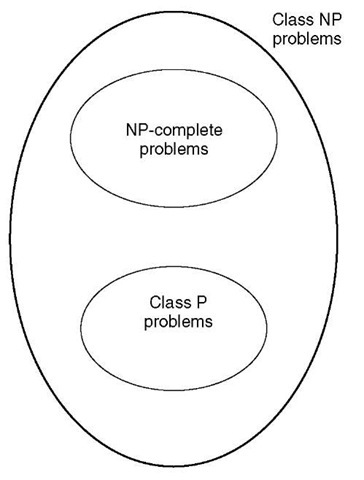
\includegraphics[width=5cm]{diagramaC}
\centering
\end{figure}
}

\frame{\titulos{El Problema SAT}{Nota sobre complejidad}
\begin{figure}[t]
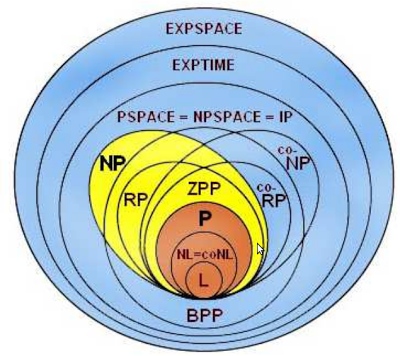
\includegraphics[width=8cm]{diagarmaC2}
\centering
\end{figure}
}

\frame{\titulos{El Problema SAT}{}
\begin{figure}[t]
\includegraphics[width=12cm]{sat}
\centering
\end{figure}
}


\frame{\titulos{Resolución Binaria}{}
\begin{block}{Resolución binaria}
Sean $\C_1,\;\C_2$ cláusulas y $\ell$ una literal. La regla de
  inferencia conocida como {\bf resolución binaria proposicional} se define como 
  sigue:
\beqs
  \frac{\C_{1} \lor \, \ell\;\;\;\;\;\; \ell^c \lor\C_2}{\C_1\lor \C_2}\;(Res)
  \eeqs
 donde $\ell^c$ es la literal contraria de $\ell$. En tal situación decimos que 
 se \textbf{resuelven} las dos premisas con respecto a la literal $\ell$ y a la 
 cláusula resultante $\C_1\lor \C_2$ se le llama {\bf resolvente o resolvente 
 binario}.
\end{block}
}

\frame{\titulos{Resolución Binaria}{}
Si bien en la definición de la regla las literales~$\ell$ y $\ell^c$ aparecen al final y principio de las cláusulas respectivamente, el orden no importa dado  que la disyunción es conmutativa. \\
\espc
\pause
\noindent Por ejemplo:
\beqs
\frac{\neg p\lor q\lor \mathbf{r} \;\;\;\;\;s\lor \mathbf{\neg r} \lor \neg t}{\neg p\lor q\lor
  s\lor \neg t}\;\;\;\;\;\;\;\;\frac{t\lor \mathbf{\neg s}\lor q\;\;\;\;\;\;\neg
q\lor w\lor \mathbf{s}\lor u}{t\lor q\lor \neg q \lor w \lor u}
\eeqs
}


\frame{\titulos{Resolución Binaria}{}
Dado que las literales también son cláusulas la aplicación
de resolución a $p$ y $\neg p$ devuelve como resultado la llamada {\bf clásula vacía}, denotada
$\square$, es decir, la siguiente es una instancia válida de resolución: 
\espc
\pause
\beqs
\frac{p\;\;\;\neg p}{\square}
\eeqs

}


\frame{\titulos{Resolución Binaria}{}
La resolución binaria proporciona un método de decisión para la lógica que utiliza el
principio de refutación para decidir la consecuencia lógica:  \\
\pause
\espc
para decidir si $\G\models\vp$ basta demostrar que $\G\cup\{\neg\vp\}$ es
insatisfacible, para lo cual basta con obtener la cláusula vacía usando la regla de resolución binaria, a partir del conjunto de cláusulas de la formas normales conjuntivas del conjunto  $\G\cup\{\neg\vp\}$.\\
\pause
\espc
 Este proceso se conoce como una {\bf refutación} del conjunto de cláusulas.\\
}


\frame{\titulos{Algoritmo de Saturación}{}
\begin{block}{n-ésima resolución}
Si $\Sg$ es cualquier conjunto de cl\'ausulas, entonces la {re\-so\-lu\-ci\'on} de $\Sg$, denotada $\mathcal{R}(\Sg)$, es el conjunto que consiste de $\Sg$ junto con todos los resolventes de cl\'ausulas de $\Sg$, es decir:
\pause
\beqs
\mathcal{R}(\Sg)=\Sg\cup \{E \, |\mbox{ existen } C,D\in\Sg\;\mbox{ tales que } E\mbox{ es
un resolvente de } C\mbox{ y } D\}.
\eeqs
\espc
\pause
La $n$-\'esima resoluci\'on de $\Sg$ se define recursivamente como sigue:
\beqs
\ba{rl}
Res_0(\Sg) &=\Sg \\
Res_{n+1}(\Sg) &=\mathcal{R}(Res_n(\Sg))
\ea
\eeqs
\espc
\end{block}
}

\frame{\titulos{Algoritmo de Saturación}{}
\begin{exampleblock}{n-ésima resolución}
Sea $\Sg$ es un conjunto finito de cl\'ausulas: \\
\espc
 $\Sg$ es no satisfacible si y s\'olo si $\square \in Res_n(\Sg)$ para alguna $n\in\mathbb{N}$.
\end{exampleblock}
\pause
\espc
Un {\bf algoritmo de saturación} se encargan de generar todos los posibles resolventes a partir de un conjunto dado $\Sg$. \\
\pause
\espc
Para verificar si un conjunto de cláusulas~$\Sg$ es {\bf insatisfacible}, basta construir con un algoritmo de saturación los conjuntos~$Res_n(\Sg)$ hasta hallar~$\square$.
}

\frame{\titulos{Algoritmo de Saturación}{}
\noindent Analicemos los escenarios posibles durante la ejecución de un algoritmo de saturación : \\
\be
\item En algún momento $\square$ es generada, es decir $\square\in Res_{n}(\Sg)$
  para algún $n\in\N$.\\ En este caso el conjunto $\Gamma$ de entrada es 
  insatisfacible. \espc
 \item El algoritmo termina sin generar~$\square$ jamás, es decir, en algún 
  momento se tiene $Res_n(\Sg)=Res_{n+1}(\Sg)$ por lo que no hay más 
  resolventes posibles, pero $\square\notin Res_n(\Sg)$.\\
  En este caso $\Gamma$ es satisfacible. 
\ee

}

\end{document}
